\chapter{\xlabel{postprocess}Post-processing Reduction Steps}
\label{sec:postprocess}

\section{\xlabel{apply_fcf}Flux-conversion factors}
\label{sec:cmult}

If you are not using the \oracdr\ pipeline to reduce your data
(i.e. you are manually employing the map-maker as described in
\cref{Chapter}{sec:manual}{Running \task{makemap} Outside the Pipeline}),
your data come out of the map-maker
in units of picowatts (pW). A flux-conversion factor, or FCF, needs to be applied to scale
your data from units of pW to janskys (Jy). For more information on
calibrating SCUBA-2 data see Dempsey et al. (2013) \cite{dempsey12},
Mairs et al. (2021) \cite{mairs21}, and \cref{Appendix}{app:cal}{SCUBA-2 data calibration}.

\vspace{5mm}

\textbf{Below are the default FCF values as of Starlink 2021A and they apply to data
obtained since 2018 June 30}. The \oracdr\ pipeline automatically accounts for changes
in the FCFs for earlier dates (see the important notes below) but manually running
the pipeline requires consulting \cref{Appendix}{app:fcfs}{FCFs by
reduction date} for the appropriate values.

\vspace{0.5cm}

\renewcommand*\arraystretch{1.2}

\begin{table}[h!]
\centering
\begin{tabular}{|c|c|c|c|}
\hline
\multicolumn{2}{|c|}{\textbf{APERTURE}}  &
\multicolumn{2}{c|}{\textbf{PEAK}}      \\
\hline
\multicolumn{2}{|c|}{\fcfa\ (Jy/pW/arcsec$^2$) }  &
\multicolumn{2}{c|}{\fcfb\ (Jy/pW/beam)}      \\
\hline
\multicolumn{1}{|c|}{450\,$\mu$m} & \multicolumn{1}{c|}{850\,$\mu$m} &
\multicolumn{1}{c|}{450\,$\mu$m}  & \multicolumn{1}{c|}{850\,$\mu$m}\\ \hline
3.87 $\pm$ 0.53                   & 2.07 $\pm$ 0.12 &
472 $\pm$ 76                      & 495 $\pm$ 32 \\
\hline
\end{tabular}
\end{table}
\renewcommand*\arraystretch{1.0}
\vspace{0.5cm}

\begin{sltextbox}{IMPORTANT NOTES:}
  \begin{itemize}
  \item The standard FCF to be applied depends on the observation date
    of your data. For data that have been \emph{reduced prior} to
    2018 June 30 you should consult \cref{Appendix}{app:fcfs}{FCFs by
      reduction date} for alternative FCFs.

  \item Due to a glitch in the WVM, data reduced between 2012
    September 19, and 2013 January 18 must be re-reduced using a
    recent version of Starlink (Hikianalia or later), or should have
    an FCF derived from a calibrator reduced at the same time (and not
    our standard FCF) applied to it. The most recent stable release of
    the Starlink software is always recommended.
  \end{itemize}
\end{sltextbox}


\subsection{Aperture flux}

To measure the flux density of extended sources with aperture photometry
you should apply the \fcfa (also known as the arcsecond FCF).
You can then sum the emission in an
aperture. \fcfa\ was determined using a 60-arcsec diameter
aperture. If your aperture differs from this you should scale your
flux accordingly---the scaling factor can be read off the curve of
growth (see \cref{Appendix}{app:cog}{this appendix}). This graph gives
the ratio of aperture flux to total flux for a range of aperture
diameters.

\fcfa\ is determined using 1-arcsec pixels. For different pixel sizes
you will also need to multiply by the pixel size squared for a total
flux calibrated in units of Jy. For more information, see
\cref{Appendix}{app:cal}{SCUBA-2 data calibration}.

\subsection{Peak flux}

If you want to read off the peak flux from your map or fit
a function to estimate the peak brightness, you should apply
the \fcfb\ (also known as the peak FCF).  When you open your map in
\gaia\ the value of the brightest pixel will be the peak flux of your
source. Applying \fcfb\ will result in a map with
units of Jy/beam. For point-like or compact sources smaller than the
beam (with a Gaussian profile), this peak value will be the total flux
density of your source. For more information, see
\cref{Appendix}{app:cal}{SCUBA-2 data calibration}.

\subsection{Manually Applying the FCF}
\label{subsec:ApplyingFCF}

You can apply an FCF value using the \picard\ recipe
\xref{\drrecipe{CALIBRATE\_SCUBA2\_DATA}}{sun265}{CALIBRATE\_SCUBA2\_DATA}.
By default, this will multiply your map by 1000$\times$\fcfb, where the default \fcfb
value is presented at the beginning of \cref{Section}{sec:cmult}{Flux-conversion factors}
or in \cref{Appendix}{app:fcfs}{FCFs by reduction date},
depending on the observation date and Starlink version used. This produces a
calibrated map with units of mJy/beam.

You can supply a parameter file if you wish to use a different value
for the FCF or use \fcfa. For example, the lines below are written in a parameter
file called \file{cal.ini} to calibrate the data \file{mapinpW.sdf} with \fcfa=2.07:

\begin{terminalv}
[CALIBRATE_SCUBA2_DATA]
FCF = 2.07
FCF_CALTYPE = ARCSEC
\end{terminalv}

The default SCUBA-2 FCF will be used if not given and FCF\_CALTYPE may either
be BEAM (default) or ARCSEC. The recipe will write out the calibrated
file with a \file{\_cal} suffix and will change the units in the map
header.

\begin{terminalv}
% picard -recpars cal.ini CALIBRATE_SCUBA2_DATA mapinpW.sdf
\end{terminalv}

Note that the recipe will also take account of the pixel size when
applying \fcfa.


\subsection{\xlabel{own_fcf}Determining your own flux-conversion factors}
\label{sec:own_fcf}

Calibration observations are obtained at various points throughout the
night and each individual observation can be used to determine FCF values.
As noted in Mairs et al. (2021)~\cite{mairs21}, the spread in FCF values observed
over periods of months or years is comparable to the scatter that can be observed
over an individual night.

There is no obvious parameter that is the singular dominant cause of the inherent scatter
in the observed FCFs. The spread is undoubtedly affected by a combination of:

\begin{enumerate}

\item The bright and variable atmosphere including subtle effects such as the
submillimeter seeing, wind speed, ambient-temperature changes, humidity and low-lying variations
in weather conditions with scale heights comparable to several times the height of the JCMT.

\item The stability of the WVM calibration.

\item Dish instability producing variations in the beam profile.

\item Instrumental noise, non-cooled optical components, and uncertainties in the {\sc{makemap}} routine's
modeling and removal of noise components from the time stream.

\end{enumerate}

We therefore recommend caution if you are calculating your own FCF
values to apply to data on a given night and suggest using the default values
supplied above or in \cref{Appendix}{app:fcfs}{FCFs by reduction date}, depending on the observation date.
Nevertheless, below are instructions on how to perform an investigation into
the FCFs calculated from the calibrator observations performed close in time
to your obtained science data:

\begin{enumerate}
\item Reduce the calibrator with the map-maker using
  \file{dimmconfig\_bright\_compact.lis} as the configuration file.

\item Determine the FCF value by passing the output map to the
  \picard\ recipe
  \xref{\drrecipe{SCUBA2\_CHECK\_CAL}}{sun265}{SCUBA2_CHECK_CAL}.

\begin{terminalv}
% picard SCUBA2_CHECK_CAL 850calibrator.sdf
\end{terminalv}

This will produce a log file (\file{log.checkcal}) which records the
both \fcfb\ and \fcfa. Check that these values closely approximate the
standard FCF values given above (to a reasonable margin within the
uncertainties).

%%
%%%%%%%
% STM - 2021, June 29. These steps don't make sense to me
% I am reframing this section as an ``Investigation of FCFs'' rather
% than advice on what to apply to data. Using DR recipes
% that were not intended for maps that have one bright
% point source in them may not accurately reflect what happens
% to fluxes in, for example, extended galactic regions as the map-maker
% models and removes noise components. Without a careful and
% controlled analysis inputting Fake sources into a variety of maps
% and comparing the results using different recipes, we should not
% give the following advice to users.
%%%%%%%
%%

%\item Re-reduce the calibrator using the map-maker with the
%  \emph{same} configuration file you used for your science
%  observations.

%\item Again determine the FCF using \drrecipe{SCUBA2\_CHECK\_CAL}.

%\item Apply this FCF to your reduced science data using \cmult---see
%  the next section. Remember to apply the pixel size squared factor if
%  using \fcfa.
\end{enumerate}


\section{\xlabel{crop}Cropping your map}
\label{sec:crop}

The nature of the scan patterns results in SCUBA-2 maps significantly
larger than the requested size. The high noise towards the outer edges
is a consequence of the scanning pattern. Although this excess data
are down-weighted during reduction by the map-maker, you may wish to
remove it before either combining maps (see
\cref{Section}{sec:coadd}{Co-adding multiple maps}) or publishing your
map.

You can crop your map to the map-size set in the data header or to any
requested size of box or circle using the \picard\ recipe
\xref{\drrecipe{CROP\_SCUBA2\_IMAGES}}{sun265}{CROP\_SCUBA2\_IMAGES}.
The centre of the cropping area will always be the centre of your map.

\begin{terminalv}
% picard -recpars mypar.lis CROP_SCUBA2_IMAGES map_cal.sdf
\end{terminalv}

The example above includes a parameter file specifying the radius of
the circle to be extracted (in arcsecs).  The format for the parameter
file is shown below.

\begin{terminalv}
[CROP_SCUBA2_IMAGES]
MAP_RADIUS = 1800.0
CROP_METHOD = circle
\end{terminalv}


If this parameter file is omitted it will default to a box of sides
equal to the map size in the header (as requested in the MSB). The
output from \drrecipe{CROP\_SCUBA2\_IMAGES} is a file with the suffix
\file{\_crop}. Full details of this recipe can be found in the
\htmladdnormallinkfoot{\textsc{Picard}
  website}{http://www.oracdr.org/oracdr/PICARD}

\begin{tip}
  The default crop shape will be a square. Avoid losing good data by
  specifying a circle using the parameter file.
\end{tip}

\section{\xlabel{coadd}Co-adding multiple maps}
\label{sec:coadd}

You may have multiple maps of the same source which you would like to
co-add. \picard\ has a recipe called
\xref{\drrecipe{MOSAIC\_JCMT\_IMAGES}}{sun265}{MOSAIC_JCMT_IMAGES}
that co-adds maps while correctly dealing with the exposure time and
weights NDF extensions. The images are combined using inverse-variance
weighting and the output variance is derived from the input variances.

\begin{terminalv}
% picard -recpars mypar.lis MOSAIC_JCMT_IMAGES 850map*_cal_crop.sdf
\end{terminalv}

This creates a single output file based on the name of the last file
in the list, and with a suffix \file{\_mos}.

There are a number of options associated with
\drrecipe{MOSAIC\_JCMT\_IMAGES} (see the \textsc{Picard} manual for a full
description). However, the main one is choosing between \wcsmosaic\
(default) and the \ccdpack\ option \makemos\ for the combination
method. For more information on \task{makemos} and advice on choosing the
best method see \xref{\textbf{SUN/139}}{sun139}{}.

The example parameter file below chooses \task{makemos} using a 3-$\sigma$
clipping threshold.

\begin{terminalv}
[MOSAIC_JCMT_IMAGES]
MOSAIC_TASK = makemos
MAKEMOS_METHOD = sigmas
MAKEMOS_SIGMAS = 3
\end{terminalv}

Currently there is no advantage in terms of data quality to reducing
all observations simultaneously or separately. However, the latter
does allow the option of assessing the individual maps before co-adding.


\subsection{Registering maps}

You can register a series of SCUBA-2 maps to a common reference
position using the \picard\ recipe
\xref{\drrecipe{SCUBA2\_REGISTER\_IMAGES}}{sun265}{SCUBA2\_REGISTER\_IMAGES}.
This is only possible if a there is a common, known source that is
present in \textit{all} of the input maps. This should be done before
combining your maps.

\begin{terminalv}
% picard -recpars myparams.ini SCUBA2_REGISTER_IMAGES -files listoffiles.txt
\end{terminalv}

Here the parameter file contains the equatorial position of the
reference source as in the example below. See \picardsun\ for more
details.

\begin{terminalv}
[SCUBA2_REGISTER_IMAGES]
REGISTER_IMAGES = 1
REGISTER_X  = HH:MM:SS.S
REGISTER_Y  = DD:MM:SS.S
\end{terminalv}

\param{REGISTER\_X} and \param{REGISTER\_Y} may also be galactic
longitude and latitude respectively, both measured in decimal
degrees.

\section{\xlabel{noise}Sensitivity}

\subsection{Getting the noise}
\label{sec:mapstats}

You can use the \picard\ recipe \drrecipe{SCUBA2\_MAPSTATS} to get the
noise. This recipe estimates the RMS from both the map, the NEP, and
the RMS predicted by the
 \href{https://www.eaobservatory.org/jcmt/instrumentation/continuum/scuba-2/itc/}{Integration
 Time Calculator}. It then writes out
a series of results in a log file called \file{log.mapstats}. The
parameters written to this file are listed in
\cref{Appendix}{app:mapstats}{SCUBA2_MAPSTATS}.

\begin{terminalv}
% picard SCUBA2_MAPSTATS map.sdf
\end{terminalv}
This recipe will report the noise in the same input units provided.


\textbf{Note:} \drrecipe{SCUBA2\_MAPSTATS} is only designed to work on
reductions of single observations. On co-added observations it could
produce misleading results, or even fail completely to work.

If multiple files are run through \drrecipe{SCUBA2\_MAPSTATS}, either in a single call
of PICARD or by repeatedly running PICARD in the same terminal on different
files, the results will be appended to the existing \file{log.mapstats} file.
The final columns — project, recipe and filename — are given to ensure it
is clear to users which line of the logfile corresponds to which input file.
This table can be viewed in an accessible way by using the \topcat\ software
included in Starlink:

\begin{terminalv}
% topcat -f ascii log.mapstats
\end{terminalv}

After running the command above, click on “Views” Then “Table Data” to display the table.

\subsubsection*{Steps for getting the noise in your co-added map}
After applying any necessary FCF, \drrecipe{SCUBA2\_MAPSTATS} simply
executes the following steps to get the map noise.

\begin{enumerate}
\item Crop the map to remove the noisy edges.

\begin{terminalv}
% picard CROP_SCUBA2_IMAGES map_cal.sdf
\end{terminalv}

\item Run the \Kappa\ command \stats\ to extract the median value from
the error array (the ndf extension that describes the uncertainty in each pixel,
calculated from the square root of the variances in the raw bolometer data
that contributed to the pixel).

\begin{terminalv}
% stats map_cal_crop comp=err order
\end{terminalv}

\end{enumerate}

\begin{tip}
  Use the error array to avoid contamination of the noise distribution
  from bright sources.
\end{tip}


\subsection{Map statistics}

The \Kappa\ commands \histat\ and \stats\ are very similar and both
return a range of statistics describing any NDF. In addition to the
main data array they can be passed the error (\param{comp=err}), variance
(\param{comp=var}) or quality (\param{comp=qua}) arrays (if available).

The reported statistics include the pixel maximum and minimum,
standard deviation, number of pixels used and omitted, along with
pixel mode, and mean.  If you supply the \xparam{ORDER}{order} keyword,
the median is also shown.

\begin{terminalv}
% stats comp=err map_cal_crop order
\end{terminalv}

\textbf{Note:} the standard deviation of the data array will give a
similar result to the mean/median of the error array except with
additional contamination from sources.



\subsection{Viewing the noise histogram}

You can view a histogram of the error array with the
\textsc{Kappa} command \histogram. Again \param{comp=err} must be
specified.

\begin{terminalv}
% histogram map_cal_crop comp=err numbin=200 style="color=white"
\end{terminalv}
The output is shown in the \cref{Figure}{fig:noihisto}{the plot below}.
For more information on the options for \histogram\ see
\kappasun.

\starfig{sc21_noihist}{}{width=0.7\linewidth}{fig:noihisto}{
  The error array viewed with \textsc{Kappa} command \task{histogram}.}{
  The error array viewed with \textsc{Kappa} command \task{histogram}.
}

\subsection{Examining the error map with GAIA}

It is also useful to view the error map itself. Open your reduced map
in \gaia, then select the \gaiathing{Error} button on the
\gaiathing{Select NDF in container file} window---see
\cref{Figure}{fig:noigaia}{the figure below}. You will need to adjust
the scaling to view the error map properly.

To assess the noise using \gaia, go to the toolbar on the main window
and click on \gaiathing{Image-Analysis$\Rightarrow$Image
regions}. Next select the region shape you would like to check and
draw it on your map by clicking and dragging the mouse. Click the
\gaiathing{Stats selected} button in the \gaiathing{Image regions}
window to get a report of the statistics in the selected region.

\begin{tip}
  You can write out the error array of your map into a new NDF using
  the \textsc{Kappa} command \ndfcopy. For example, \texttt{\% ndfcopy
    map comp=err map\_err}
\end{tip}



\starfig{sc21_noigaia6}{[h!]}{width=\linewidth}{fig:noigaia}{
  The error map viewed with \gaia}{
  The error array displayed with \gaia. After clicking the
  \gaiathing{Error} button (circled in red) you will have to rescale your map.
}


\section{\xlabel{regridding}Regridding your data}
\label{sec:regriddata}

To change the pixel size use the \Kappa\ command \compave. The
following example increases the pixel size from 4\,arcsec to 8\,arcsec
by using a compression factor of 2.

\begin{terminalv}
% compave map map_regrid 2
\end{terminalv}

\begin{tip}
  Remember you can use \ndftrace\ if you are unsure of the pixel size.
\end{tip}


% they find that smaller pixels produce higher peak values (due to the
% smaller pixels producing less smoothing that larger pixels), and
% also converge faster (due to each pixel needing to be consistent
% with fewer bolometers). The average noise per pixel is higher for
% smaller pixels (as expected), and this means that the SNR level used
% for masking needs to be adjusted to get the same mask produced using
% larger pixels.

\section{\xlabel{maskshow}Displaying masks}
\label{sec:maskshow}

SCUBA-2 maps created using ``\model{AST}-masking'' (see \cref{Section}
{sec:masking}{Masking}) will contain a \texttt{Quality} array indicating the
background pixels that were masked (i.e. forced to zero). In itself this
is fairly simple---background pixels have a non-zero Quality value and
source pixels have a Quality value of zero. However, it is also possible
to have independent masks for the \model{FLT} and \model{COM} models,
in addition to the \model{AST} mask. For instance, maps created using
\brightextended\ or \jsageneric\ will have \texttt{Quality} arrays that
contain both a \model{FLT} and an \model{AST} mask, and so some care needs
to be used when interpreting the \texttt{Quality} array.

Each value in the \texttt{Quality} array is restricted to taking integer values
between 0 and 255, and so can be thought of as 8 separate bits. Each ``bit
plane'' within the \texttt{Quality} array holds a single mask---\model{AST},
\model{FLT} or \model{COM}. The \xref{\task{showqual}}{sun95}{SHOWQUAL}
command can be used to find out which mask is held by which bit plane:

\begin{terminalv}
% showqual fred.sdf
   AST (bit 1) - "Set iff AST model is zeroed at the output pixel"
   FLT (bit 2) - "Set iff FLT model is blanked at the output pixel"
\end{terminalv}

This means that the \model{AST} mask is stored in bit 1 (the least significant
bit), the \model{FLT} mask is stored in bit 2, and there is no \model{COM}
mask. Note, if
a map was produced using \model{FLT} masking but no \model{AST} masking,
then the \model{FLT} mask would be stored in bit 1.

The decimal integer value of any element of the \texttt{Quality} array is
equal to the binary value formed from the bits listed by \task{showqual}.
So in the above case the maximum \texttt{Quality} value is 3 (the decimal
equivalent of binary ``11''-e--both bits set). Remembering that a bit is set
(\emph{i.e.} is 1) for background pixels and cleared (\emph{i.e.} is 0) for
source pixels, it follows that the four possible decimal \texttt{Quality}
values in the above case (0-3) are:

\begin{enumerate}
\item - neither bit set, so the pixel is inside both the \model{AST} and the \model{FLT} mask
(a source pixel).

\item -- Bit 1 set, but not Bit 2, so the pixel is outside the \model{AST} mask but
inside the \model{FLT} mask (a border-line pixel).

\item -- Bit 2 set, but not Bit 1, so the pixel is inside the \model{AST} mask but
outside the \model{FLT} mask (a border-line pixel).

\item -- Both bits set, so the pixel is inside neither mask (a background
pixel).
\end{enumerate}

\cref{Figure}{fig:qualmap}{Quality component displayed as an image} shows
a simple map of the \texttt{Quality} array values---the black areas have
value zero and are thus inside both masks, the dark brown areas have value 2
and are thus inside the \model{AST} mask but outside the \model{FLT} mask.
The light-brown areas have value 3 and are inside neither mask. In this
particular case, there are no  areas with a quality value of 1, so the
\model{FLT} mask is contained entirely within the \model{AST} mask.

\begin{figure}[t!]
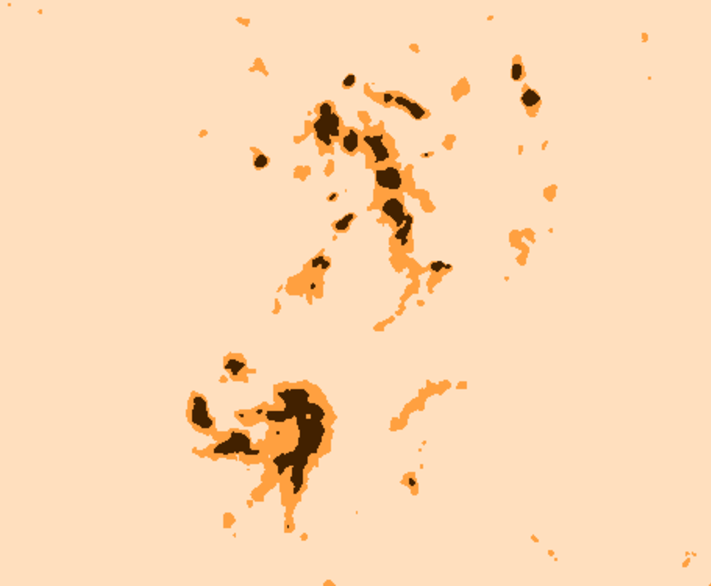
\includegraphics[width=0.6\linewidth]{sc21_qual}
\caption[Quality component displayed as an image]{The quality component
from a typical map.}
\label{fig:qualmap}
\end{figure}

To produce a plot like this, first open your map in \textsc{Gaia}. Select
the top level NDF from list in the pop-up window then click the
\gaiathing{Quality} button. You will need to rescale the map to bring
out the masks--see \cref{Figure}{fig:qualdisp}{} for another example
showing the full \textsc{Gaia} window (using rather brighter colours this
time!).

\starfig{sc21_qualitygaia}{[t!]}{width=0.9\hsize}{fig:qualdisp}{
   Display of the mask made by the map-maker}{
   Using \gaia\ to display the mask applied by the map-maker. Select the
   QUALITY component of your map.
}

There are several commands within \textsc{Kappa} that manipulate
\texttt{Quality} arrays in various ways. For instance, the
\xref{\task{setbb}}{sun95}{SETBB} command allows pixel data values to
be set bad if the associated \texttt{Quality} value has a specified
collection of set bits. Thus:

\begin{terminalv}
% setbb fred 1
\end{terminalv}

will set all pixels bad in \texttt{fred.sdf} except for those inside the
\model{AST} mask. Likewise,

\begin{terminalv}
% setbb fred 2
\end{terminalv}

will set all pixels bad except for those inside the \model{FLT} mask.  Note, the
change made by \task{setbb} is temporary---it can be undone by doing:

\begin{terminalv}
% setbb fred 0
\end{terminalv}

To display the \texttt{fred.sdf} map and then overlay the \model{AST} mask in blue
and the \model{FLT} mask in red, do:

\begin{terminalv}
% gdclear
% display fred mode=perc percentiles=\[2,98\]
% setbb fred 1
% contour fred clear=no mode=good labpos=! style='colour=blue'
% setbb fred 2
% contour fred clear=no mode=good labpos=! style='colour=red'
% setbb fred 0
\end{terminalv}

The resulting plot is shown in \cref{Figure}{fig:masks}{AST and FLT masks
shown together}.

\begin{figure}[t!]
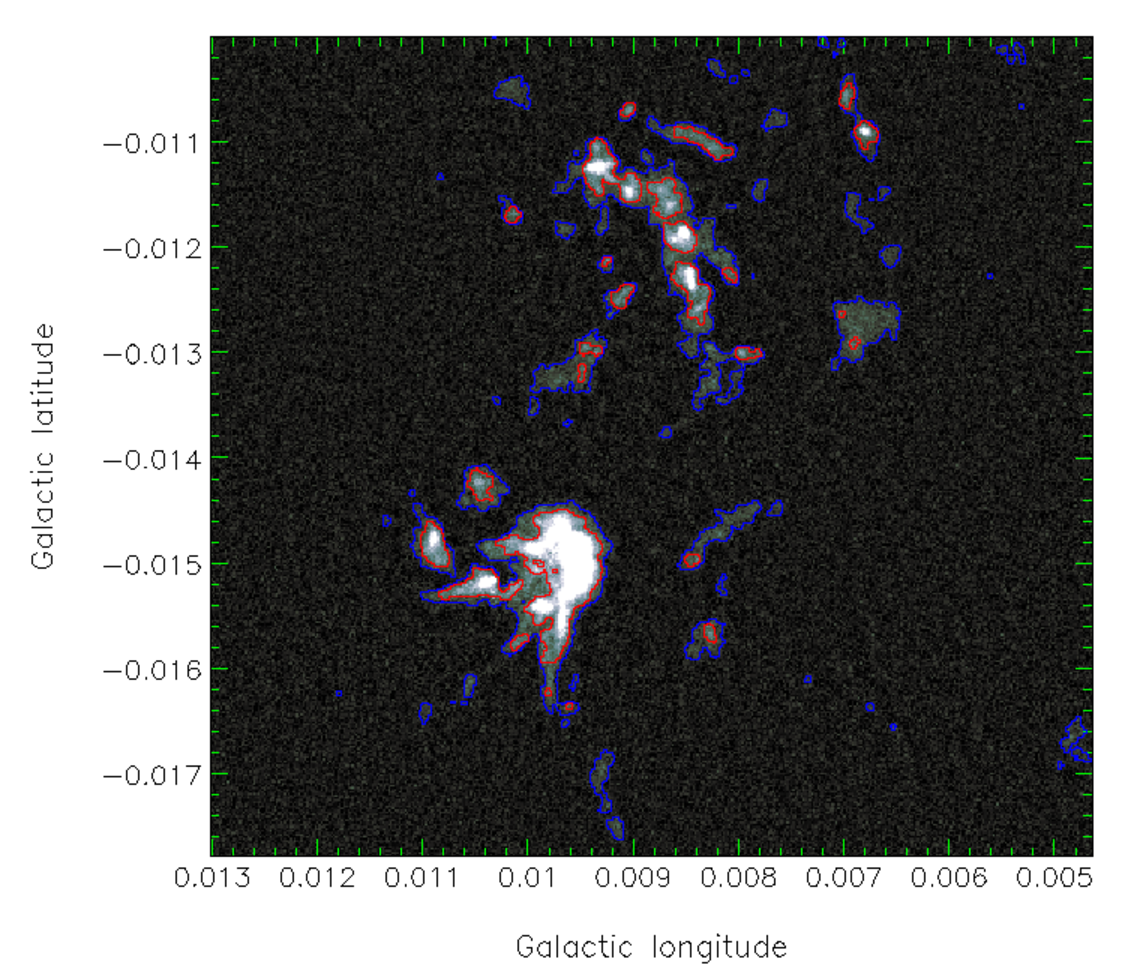
\includegraphics[width=0.6\linewidth]{sc21_masks}
\caption[AST and FLT masks shown together]{The AST and FLT masks contoured
together over an image.}
\label{fig:masks}
\end{figure}

Alternatively, \gaia\ can be used to contour the \texttt{Quality} array
over an image, but you cannot then distinguish the \model{AST} mask from
the \model{FLT} mask. First you will need to copy out the QUALITY component
of the data to a separate file using \task{ndfcopy}:

\begin{terminalv}
% ndfcopy comp=qua map map_mask
\end{terminalv}

Then open your map in \gaia\ and contour the mask NDF on top.
Select \gaiathing{Contouring...} from the \gaiathing{Image-Analysis}
menu, and supply the name of the mask NDF either by entering its name in
the \gaiathing{Other image:} box, or selecting with
\gaiathing{Choose file...} file browser. See
\cref{Figure}{fig:maskdisp}{the figure below}.

For more information on the use of masks by \makemap\ and the
parameters that affect them see \cref{section}{sec:masking}{Masking}.

\starfig{sc21_dispmask3}{[hb!]}{width=0.95\linewidth}{fig:maskdisp}{
   Contours of an \model{AST} mask overlaid on a map}{
   Using \gaia\ to display your map with the \model{AST} mask used by
   the map-maker contoured on top.
}


\section{\xlabel{match_filter}Point-source extraction: the matched filter}
\label{sec:mf}

This effectively fits a single Gaussian point spread function (PSF),
centered over every pixel in the map, and applies a background
suppression filter to remove any residual large-scale noise.

Cosmology maps usually contain very faint sources that often need
extra help extracting. The \picard\ recipe
\xref{\drrecipe{SCUBA2\_MATCHED\_FILTER}}{sun265}{SCUBA2_MATCHED_FILTER}
can be used to improve point-source detectability.

The matched filter works by smoothing the map and PSF with a broad
Gaussian, and then subtracting from the originals. The images are then
convolved with the modified PSF. The output map should be used
primarily for source detection only. Although the output is normalised
to preserve peak flux density, the accuracy of this depends on how
closely the real PSF matches the telescope beam size. In the case of
nearby sources, each ends up contributing flux to both peaks.

\begin{terminalv}
% picard -recpars mypar.lis SCUBA2_MATCHED_FILTER 850_map_cal_crop.sdf
\end{terminalv}

As in the example parameter file below we have requested the
background should be estimated by first smoothing the map and PSF with
a 15-arcsec Gaussian.

\begin{terminalv}

[SCUBA2_MATCHED_FILTER]
SMOOTH_FWHM = 15

\end{terminalv}

This is a fairly common technique used throughout the extra-galactic
sub-millimetre community to identify potential sources. A full
description of the matched filter principle is given in
\cref{Appendix}{app:mf}{SCUBA-2 matched filter}, while the
\textsc{Picard} manual gives full details of all the available
parameters.

\section{\xlabel{clumps}Clump finding}
\label{sec:clumps}
\label{sec:clumpfind}

The \cupid\ application \findclumps\ can be used to generate a clump
catalogue. It identifies clumps of emission in one-, two- or
three-dimensional NDFs. You can select from the clump-finding
algorithms ``FellWalker''\cite{fellwalker}, ``Gaussclumps'',
``ClumpFind'' or ``Reinhold'' and must supply a configuration file
specific to each method. See the \xref{\textsc{Cupid} manual}{sun255}{}
for descriptions of the various algorithms.

The result is returned as a catalogue in a text file and as a NDF
pixel mask showing the clump boundaries.

\begin{terminalv}
% findclumps in=S2map.sdf out=clumpmap.sdf outcat=clumps.FIT logfile=clumps.log \
  config=^config.dat method=fellwalker rms=25 shape=polygon
\end{terminalv}

The shape option allows \findclumps\ to create an
\htmladdnormallink{STC-S}{http://ivoa.net/documents/STC-S/index.html}
description (polygonal or elliptical) for each clump that
can be displayed over any image in \gaia (\cref{Figure}{fig:stcshapes}{}).
These are added as extra columns to the output catalogue.

\begin{aligndesc}
\item[Polygon] Each polygon will have, at most, 15 vertices. For
  two-dimensional data the polygon is a fit to the clump's outer
  boundary (the region containing all good data values). For
  three-dimensional data the spatial footprint of each clump is
  determined by rejecting the least significant 10\% of spatial
  pixels, where "significance" is measured by the number of spectral
  channels that contribute to the spatial pixel. The polygon is then a
  fit to the outer boundary of the remaining spatial pixels.

\item[Ellipse] All data values in the clump are projected onto the
  spatial plane and "size" of the collapsed clump at four different
  position angles---all separated by 45$^\circ$---is found. The
  ellipse that generates the same sizes at the four position angles is
  then found and used as the clump shape.
\end{aligndesc}

\starfig{sc21_plotstcshapes}{[ht!]}{width=1.0\linewidth}{fig:stcshapes}{
  Overlaying a clump catalogue in \gaia.}{
  STC shapes displayed over the input map with \gaia. To overlay your clumps
  in this way display your map with \textsc{Gaia}. Under the \gaiathing{Image-Analysis}
  menu select \gaiathing{Positions...} followed by \gaiathing{Import CUPID
  catalogue...} In the pop-up window select the \file{.FIT} file
  generated by \findclumps\ and ensure the \gaiathing{STC shape} box is
  checked before importing.
}


\section{\xlabel{provenance}Map provenance \& configuration parameters}
\label{sec:prov}

You may want to check a reduced file to determine which raw files went
into it and what configuration parameters were used with the
map-maker. There are a number of useful \Kappa\ commands to help you
with this:

\begin{description}
\item[Map provenance]
  \provshow\ will list all the NDFs and operations that were used in the
  creation of your map, while \hislist\ will show a truncated list of input
  files and operations but will list every configuration parameter used by
  the map-maker.  This includes all the hidden default values as well as
  those specified in your supplied configuration file. These commands are
  executed like this:

\begin{terminalv}
% provshow 850map
% hislist 850map
\end{terminalv}

The output of \task{provshow} can be very long.  If you merely want to
know what the original files were, the ones with no parents, select the
root ancestors.

\begin{terminalv}
% provshow 850map show=roots
\end{terminalv}


\item[Map-maker parameters]
The task \configmeld\ will compare two maps and highlight any differences
between the configuration parameters that were used to create the maps. A
configuration file can be supplied in place of a map, in which case the
parameters used to create the map are compared with those in the
configuration file. \task{configmeld} requires a visual-differences tool
to be installed on your machine; those currently recognised are:
\htmladdnormallink{\texttt{meld}}{http://meldmerge.org/}
\htmladdnormallink{\texttt{opendiff}}{http://developer.apple.com/},
\htmladdnormallink{\texttt{diffmerge}}{http://www.sourcegear.com/diffmerge},
\htmladdnormallink{\texttt{kdiff3}}{http://kdiff3.sourceforge.net},
\htmladdnormallink{\texttt{tkdiff}}{http://sourceforge.net/projects/tkdiff}, and
\htmladdnormallink{\texttt{diffuse}}{http://diffuse.sourceforge.net},
and are searched for in that order. The follow example illustrates two
ways to run \task{configmeld}:

\begin{terminalv}
% configmeld 850map1.sdf 850map2.sdf
% configmeld 850map1.sdf ^mydimmconfig2.lis
\end{terminalv}

Another useful command is the \Kappa\ command \configecho.
This is very versatile and will display the name and value of one or
all configuration parameters either from a configuration file or from
the history of an NDF.

The first example below will return the value of \xparam{NUMITER}{numiter} from
the map \file{850map.sdf}. The second example will display the values of all
the parameters in \file{850map.sdf} and will prefix them with a `+' if they
differ from the the default parameter values defined in \file{\$SMURF\_DIR/smurf\_makemap.def}.

\begin{terminalv}
% configecho name=numiter config=! ndf=850map.sdf
% configecho name=! config=^$SMURF_DIR/smurf_makemap.def ndf=850map.sdf
\end{terminalv}
\end{description}


